\chapter{Anhang}

\section{Umfrage}
\subsection{Interview-Leitfaden}\label{subsec:leitfaden}
Vielen Dank, dass sie sich Zeit genommen haben, in dieser Evaluation zur Benutzerfreundlichkeit von flowws teilzunehmen.

flowws ist eine Softwareumgebung, die es sich zum Ziel gesetzt hat, die Programmierung von Smart Devices und Connected Products (bspw. NEST-Thermostat, Fitbit, Hue Glühbirnen, etc.) zu erleichtern und auch Nicht-Technikern zu ermöglichen. Um dieses Ziel zu erreichen, wird flowws in Verbindung mit cBlocks verwendet, um Prototypen im \ac{IoT} Bereich zu erstellen. Zwar besitzen diese Prototypen nicht das Aussehen des finalen Produkts, sollen aber das gleiche Verhalten abbilden. 

cBlocks sind physikalische Bausteine, welche die einzelnen Elektronikbausteine repräsentieren, aus denen sich Smart Devices zusammensetzen: Sensoren und Aktoren. cBlocks spalten sich in zwei Gruppen auf:
\begin{itemize}
    \item \textbf{Sensor-cBlocks} transformieren physische Signale (Licht, Schall, Temperatur, etc.) in elektronische Signale um.
    \item \textbf{Aktor-cBlocks} sind bspw. Lautsprecher und LEDs. Sie wandeln elektronische Signale in physikalische Signale (LED aufleuchten, mit Lautsprecher Geräusch abspielen, etc.) um.
\end{itemize}
Ein Beispiel für einen Prototyp könnte ein intelligenter Rauchmelder sein. Ein solcher Rauchmelder würde aus drei cBlocks gebaut werden, welche CO2-Sensor, Temperatur-Sensor und Lautsprecher-Aktor besitzen. Die Logik nach der sich der Rauchmelder verhält muss ihm einprogrammiert werden. Hierbei kommt flowws ins Spiel.

flowws verbindet Sensor- und Aktor-cBlocks, indem es die Daten, welche die Sensoren erzeugen umwandelt, und damit das Verhalten der Aktoren steuert. Für die Umwandlung von Daten kommt eine dritter, rein virtueller, Block zum Einsatz: der Wandler/Transducer. Ein Wandler würde im oberen Beispiel die Temperatur-Daten und CO2-Konzentration der Sensor-cBlocks kombinieren und darüber entscheiden ob der Lautsprecher-cBlock Alarm schlagen soll.

Der Nutzer verwendet flowws, um genau diese Art von Logik auf einer graphischen Oberfläche zu programmieren.

Uns interessiert die Verständlichkeit von flowws. Aus diesem Grund, werden dir im Folgenden mehrere Programme in flowws gezeigt. Wobei es deine Aufgabe ist, die Funktionen der einzelnen Elemente, ihre Aufgaben zu deuten und ihr Verhalten vorherzusagen.

\subsection{Fragebogen}\label{subsec:fragebogen}
\begin{table}[H]
\caption{Angaben zur Person}
\label{tab:questPers}
\begin{tabularx}{\textwidth}{lX}
\hline
\rowcolor[HTML]{EFEFEF} 
Charakteristik                              & Ausprägung                                \\ \hline
Name                                        &                                           \\ \hline
Geschlecht                                  &                                           \\ \hline
Alter                                       &                                           \\ \hline
Beruf/Studium                               &                                           \\ \hline
\end{tabularx}
\end{table}


\begin{table}[H]
\caption{Angaben zur Erfahrungen}
\label{tab:questErf}
\begin{tabularx}{\textwidth}{Xccc}
\hline
\rowcolor[HTML]{EFEFEF} 
Erfahrung mit...                              & & Ausprägung                             &   \\ \hline
...IoT & unbedarft & \Circle \: \Circle \: \Circle \: \Circle \: \Circle \: \Circle & selbst schon entwickelt  \\ \hline
...Designmethoden & unbedarft & \Circle \: \Circle \: \Circle \: \Circle \: \Circle \: \Circle & Designexperte  \\ \hline
...Software-Engineering & unbedarft & \Circle \: \Circle \: \Circle \: \Circle \: \Circle \: \Circle & Informatik Studium \\ \hline
...Zustandsautomaten & unbedarft & \Circle \: \Circle \: \Circle \: \Circle \: \Circle \: \Circle & schon Programmiert \\ \hline
...Datenfluss-Programmierung & unbedarft & \Circle \: \Circle \: \Circle \: \Circle \: \Circle \: \Circle & schon Programmiert \\ \hline
\end{tabularx}
\end{table}

\newpage

\subsubsection{Fragen zu Szenarios}
Welche Komponenten sehen sie im Programm?\\
\noindent\rule{\textwidth}{1pt}
\noindent\rule{\textwidth}{1pt}
\noindent\rule{\textwidth}{1pt}

Welche Aufgaben haben diese Komponenten? Wie reagieren sie auf eingehende Signale?\\
\noindent\rule{\textwidth}{1pt}
\noindent\rule{\textwidth}{1pt}
\noindent\rule{\textwidth}{1pt}

Was ist der Aktor wie verhält er sich auf eingehende Signale? Welche sendet er aus?\\
\noindent\rule{\textwidth}{1pt}
\noindent\rule{\textwidth}{1pt}
\noindent\rule{\textwidth}{1pt}

Wann hat das Programm entgegen ihren Vermutungen gehandelt?\\
\noindent\rule{\textwidth}{1pt}
\noindent\rule{\textwidth}{1pt}
\noindent\rule{\textwidth}{1pt}

\newpage
\subsubsection{Generelle Fragen}
\textbf{Diffuseness}: Sagen Programme in flowws direkt, was sie machen?\\
\noindent\rule{\textwidth}{1pt}
\noindent\rule{\textwidth}{1pt}
\noindent\rule{\textwidth}{1pt}

\textbf{Closeness o. M.}: Inwieweit unterscheidet sich die Notation des flowws-\\Programms, von ihren Erwartungen?\\
\noindent\rule{\textwidth}{1pt}
\noindent\rule{\textwidth}{1pt}
\noindent\rule{\textwidth}{1pt}

\textbf{Role-Express.}: Konnten sie die Aufgaben der einzelnen Komponenten im Gesamtkontext deuten?\\
\noindent\rule{\textwidth}{1pt}
\noindent\rule{\textwidth}{1pt}
\noindent\rule{\textwidth}{1pt}

\textbf{Prog Eval}: Hat es flowws ihnen ermöglicht zu jeder Zeit nachzuvollziehen, wie das Ergebnis des Programmes ist.\\
\noindent\rule{\textwidth}{1pt}
\noindent\rule{\textwidth}{1pt}
\noindent\rule{\textwidth}{1pt}

\textbf{Impro}: Denken sie es gibt konkrete Möglichkeiten flowws zu verbessern? Wenn ja, wie?\\
\noindent\rule{\textwidth}{1pt}
\noindent\rule{\textwidth}{1pt}
\noindent\rule{\textwidth}{1pt}
\newpage

\subsection{Szenario \#1}\label{anhang:szenario1}
\begin{figure}[H]
    \centering
    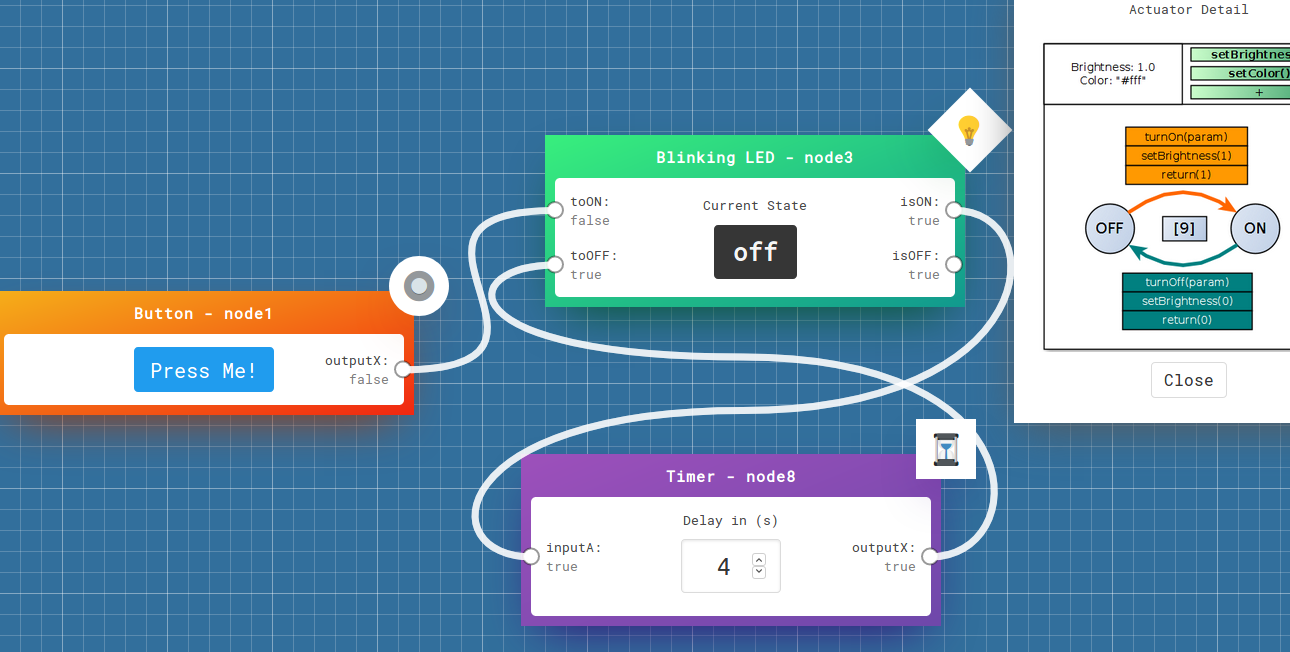
\includegraphics[width=1\textwidth]{bilder/Anhang/timerclock_cut.png}
    \caption{Szenario \#1: Bestehend aus Taster-Sensorknoten, LED-Aktorknoten und Timer-Funktionsknoten.}
    \label{fig:szenario1}
\end{figure}
Dieser Graph (siehe \ref{fig:szenario1}) bildet die Zeitschaltuhr aus Szenario \#1 (siehe Kapitel \ref{szenario1}) ab. Das Szenario besteht aus drei Elementen und verwendet dabei jeden Typ von Knoten. 
Ziel dabei ist es, das der Endnutzer die einzelnen Elemente identifiziert und ihr Zusammenspiel erklärt. Es ist insbesondere interessant, ob der Proband realisiert, dass der Aktor seinen Zustand dem Rest des Graphen mitteilt und somit das Verzögerte ausschalten der LED ermöglicht.

\subsection{Szenario \#2}\label{anhang:szenario2}
\begin{figure}[H]
    \centering
    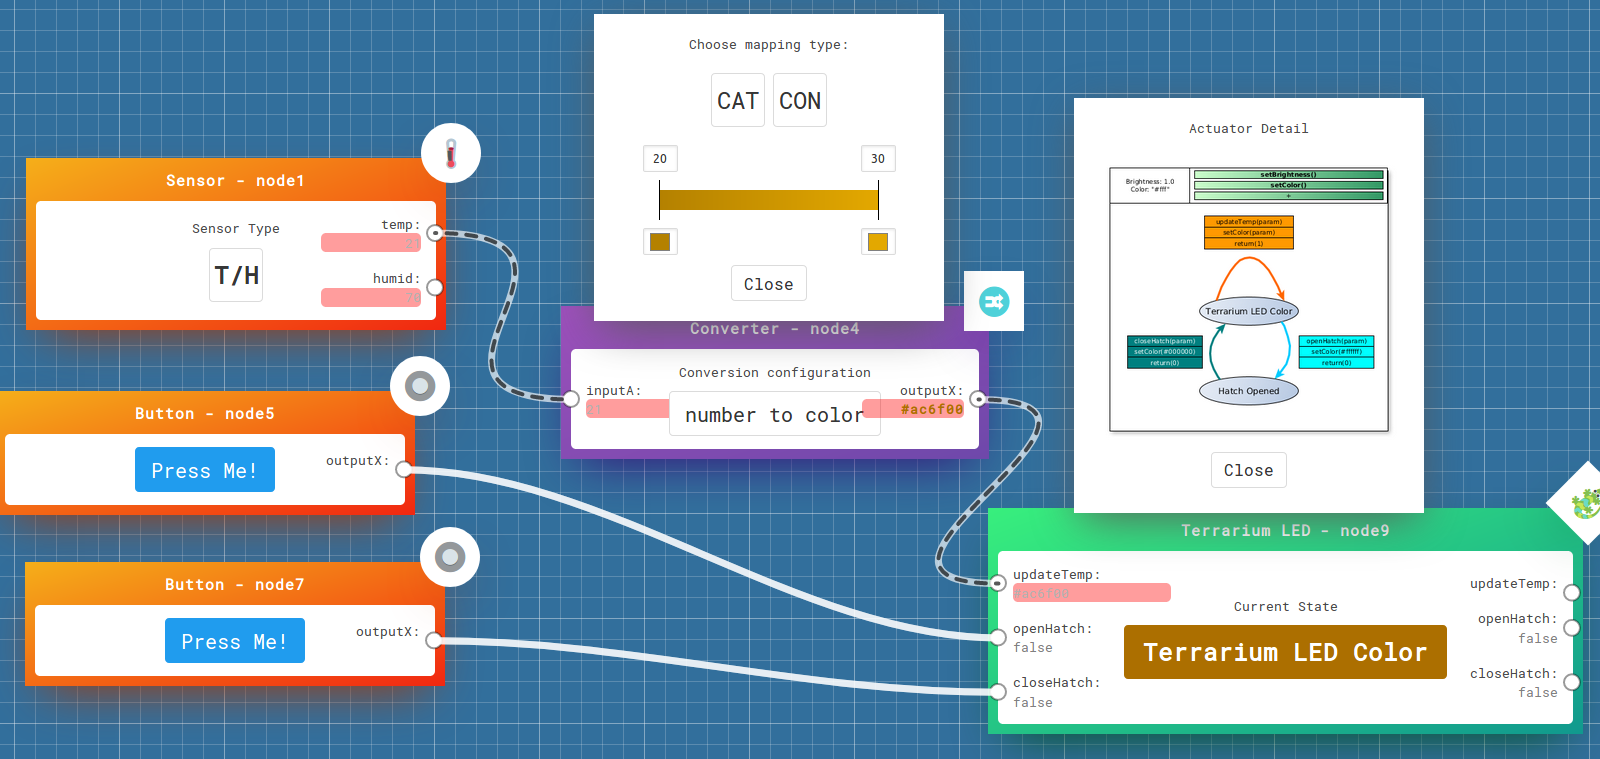
\includegraphics[width=1\textwidth]{bilder/Anhang/terrariumszenario_cut.png}
    \caption{Szenario \#2: Bestehend aus zwei Taster-Sensorknoten, LED-Aktorknoten und Konverter-Funktionsknoten}
    \label{fig:szenario3}
\end{figure}
In Abbildung \ref{fig:szenario3} wird das Terrarium Szenario \#3 von Kapitel \ref{szenario3} im flowws-Prototyp abgebildet. Das Terrarium regelt die Helligkeit abhängig von der Temperatur innerhalb des Terrariums automatisch.
Wird das Terrarium geöffnet, wird ein Taster betätigt und erhellt sich das Terrarium auf die maximale Stufe. Sobald das Terrarium wieder geschlossen wird, wird ein zweiter Taster betätigt und das Terrarium regelt sich wieder anhand des Temperatur-Sensors. 

Der Proband muss hierbei, wie im vorherigen Beispiel, die einzelnen Knoten identifizieren. Gleichzeitig soll der Proband die komplexere Aktorlogik verstehen. Dazu gehört, dass der LED-Aktor eine Signalpriorisierung vornimmt, sobald das Terrarium geöffnet ist.
\newpage